\documentclass[a4paper]{article}


\usepackage[margin=1in]{geometry} % full-width

% AMS Packages
\usepackage{amsmath}
\usepackage{amsthm}
\usepackage{amssymb}

% Unicode
\usepackage[utf8]{inputenc}
\usepackage{hyperref}
\hypersetup{
	unicode,
	pdfauthor={María San José Seco},
	pdftitle={Estudio práctico de técnicas de ofuscación y contramedidas aplicables},
	pdfsubject={Estudio práctico de técnicas de ofuscación y contramedidas aplicables},
	pdfkeywords={obfuscation, malware, javascript},
	pdfproducer={María San José},
	pdfcreator={María San José}
}


% Natbib
\usepackage[sort&compress,numbers,square]{natbib}
\bibliographystyle{mplainnat}


\usepackage{graphicx, color}
\graphicspath{{fig/}}

\usepackage[spanish]{babel}

\usepackage{algorithm, algpseudocode} % use algorithm and algorithmicx for typesetting algorithms
\usepackage{mathrsfs} % for \mathscr command

\usepackage{lipsum}

\usepackage{fancyhdr}
\pagestyle{fancy}
\fancyhead{} % clear all header fields
\fancyhead[R]{\textbf{TFM: Estudio práctico de técnicas de ofuscación y contramedidas aplicables}}
\fancyfoot{} % clear all footer fields
\fancyfoot[R]{\thepage}

% Author info
\title{Estudio práctico de técnicas de ofuscación y contramedidas aplicables}
\author{María San José Seco \\ \href{https://github.com/drkrysSrng/freyja}{@drkrysSrng/freyja}}

\date{
	Universidad Católica de Murcia \\
	ENIIT - Campus Internacional de Ciberseguridad
}

\begin{document}

	\maketitle
	
	\section{Introducción}
		
	A lo largo de la historia, tanto como para proteger la propiedad intelectual o intercambiar secretos, se ha utilizado la ofuscación como medida de protección. El malware la ido evolucionando a través de los años utilizando diferentes técnicas cada vez más avanzadas de manera que los antivirus y los analistas no puedan detectarlos y evadirlos, ya que este método previene los análisis por firma o hash o por las reglas YARA que ayudan a buscar cadenas de texto sospechosas dentro de ellos. 

	Hoy en día, el tipo de malware que más nos podemos encontrar, es metamórfico, ya que se ha avanzado mucho para evadir los antivirus. De esta manera, la evolución del malware parte desde el punto de encontrarnos muestras oligomórficas, donde la parte viral está encriptada, muestras polimórficas, donde no soĺo está encriptado sino que también está ofuscado. El primer malware polimórfico de la Historia, Luna fue desarrollado en España por Bumblebee en el año 1999. 
	
	
	Analizar la Entropía de una muestra es importante, de esa manera,  se puede identificar la aleatoriedad o desorden de un sistema, de manera que podamos identificar si una muestra ha sido ofuscada o no. Cuanto más alta sea la probabilidad y sobre todo mayor de \textit{3.75} significa que no ha sido escrito por un humano.
	
	\section{Importancia de las amenazas de JavaScript en Windows}
	Los ataques basados en script se han convertido en una amenaza importante en los últimos años. Siendo el 40\% de los últimos años, entre los lenguajes más utilizados se encuentran PowerShell, VBScript y JavaScript. Sin embargo la mayoría de malware se están migrando a éste último ya que es un lenguaje que se puede ejecutar dentro y fuera del navegador en sistemas Windows.
	
	
	\section{Freyja Deobfuscation Tool }
	\href{https://github.com/drkrysSrng/freyja}{@drkrysSrng/freyja}
	
	Se ha desarrollado la siguiente herramienta para aplicar varios tipos de ofuscación mencionados en el apartado anterior:
	
	\begin{itemize}
		\item Limpia el código y lo tabula de manera similar, no sólo tabulando las instrucciones, sino que parsea los caracteres en hexadecimal y unicode.
		\item Chequeeo de la entropía con el algoritmo de Shannon, línea por línea o por texto completo.
		\item Cuando los caracteres Unicode o en Hexadecimal no están parseados ya que no están en formato String sino que es una variable ofuscada, se parsean a mayores también.
		\item Desofusca funciones como \verb*|toString|, conjuntos de números dentro de \verb*|eval|, sustituir \verb*|unescape| y \verb*|parseint|:
		\item Concatena cadenas de caracteres separadas con el símbolo \verb*|+|
		\item Búsqueda de strings en base64 y su decodificación.
	\end{itemize}

	\begin{figure}[H]
		\centering
		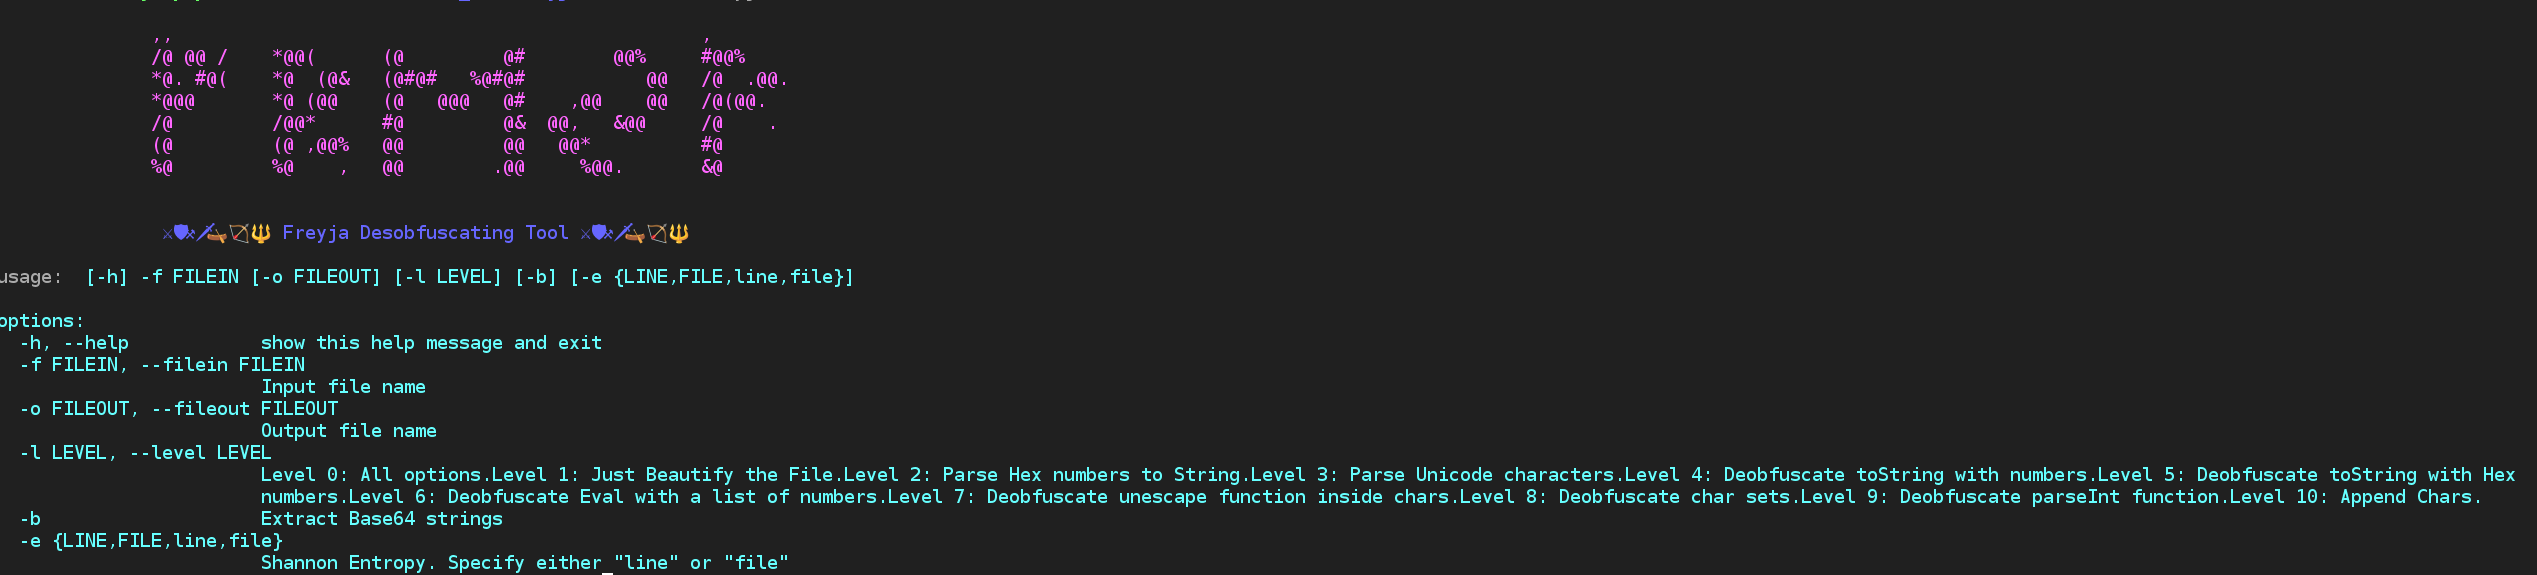
\includegraphics[width=18cm]{images/usage.png}
		\caption{Uso de la herramienta Freyja}
	\end{figure}
	
	\begin{itemize}
		\item \verb*|-f| Fichero a desofuscar.
		\item \verb*|-o| Fichero de salida desofuscado.
		\item \verb*|-l| Nivel de ofuscación. Le indicamos la técnica que queremos que utilice.
		\begin{itemize}
			\item Nivel 0: Todas las opciones
			\item Nivel 1: Técnica \textit{beautify}, tabular el fichero y darle formato al JavaScript.
			\item Nivel 3: Parsear los caracteres Unicode a Strings.
			\item Nivel 4: Desofuscar la función \verb*|toString|.
			\item Nivel 5: Desofuscar la función  \verb*|toString| con número hexadecimal.
			\item Nivel 6: Desofuscar la función  \verb*|eval| cuando tiene una lista de números.
			\item Nivel 7: Desofuscar la función  \verb*|unescape| cuando contiene caracteres.
			\item Nivel 8: Desofuscar conjuntos de caracteres.
			\item Nivel 9: Desofuscar la función  \verb*|parseInt|.
			\item Nivel 10: Concatena caracteres aunque estén en varias líneas.
		\end{itemize}
	\end{itemize}
\end{document}

